\documentclass[11pt]{article}

% ----- Packages -----
\usepackage{amsmath, amssymb, amsthm, geometry, mathrsfs, mathtools}
\usepackage{tikz}
\usetikzlibrary{arrows.meta, positioning, shapes.geometric, backgrounds, patterns}
\usepackage{hyperref}
\usepackage{enumitem}

% ----- Page Setup -----
\geometry{letterpaper, margin=1in}
\setlength{\parindent}{0pt}
\setlength{\parskip}{0.6em}

% ----- Theorem Environments -----
\newtheorem{theorem}{Theorem}[section]
\newtheorem{lemma}[theorem]{Lemma}
\newtheorem{proposition}[theorem]{Proposition}
\newtheorem{corollary}[theorem]{Corollary}
\newtheorem{definition}{Definition}[section]
\newtheorem{axiom}{Axiom}[section]

\theoremstyle{remark}
\newtheorem*{remark}{Remark}
\newtheorem*{solution}{Solution}

% ----- Title Information -----
\title{\textbf{Homework 3.1 \& 3.2: Direct Proof, Trivial, and Vacuous Proofs}}
\author{Tashfeen Omran}
\date{September 2026}

\begin{document}

\maketitle
\tableofcontents
\newpage

% =======================================================================
\section{Part 1: Comprehensive Introduction, Context, and Prerequisites}
% =======================================================================

\subsection{Historical Context and Motivation}
In the late 19th and early 20th centuries, the foundational crisis of mathematics—driven by paradoxes such as Russell's Paradox—compelled mathematicians like Gottlob Frege, Bertrand Russell, and David Hilbert to construct an airtight framework for logical deduction. This era solidified formal logic and set theory as the bedrock of mathematical rigor. A key outcome of this formalization was the rigorous definition of material implication, $P \implies Q$. In everyday language, we often assume a causal relationship between $P$ and $Q$. However, in formal mathematics, material implication is evaluated purely functionally via truth tables, giving rise to counterintuitive yet logically sound constructs: the \textit{vacuous proof} and the \textit{trivial proof}. Understanding these techniques is not just an exercise in semantics; it forms the backbone of boundary-case analysis in algorithmic verification, measure-theoretic probability (where probability-zero events conceptually mirror vacuous truths), and structural induction.

\subsection{Core Concepts, Axioms, and Definitions}
At the heart of Sections 3.1 and 3.2 is the logical structure of an implication over a domain $S$. 
Let $P(x)$ and $Q(x)$ be open sentences over a domain $S$. We are evaluating the quantified statement:
\[ \forall x \in S, \ P(x) \implies Q(x) \]

\begin{definition}[Material Implication]
The implication $P \implies Q$ is false if and only if $P$ is true and $Q$ is false. In all other cases—namely, when $P$ is true and $Q$ is true, when $P$ is false and $Q$ is false, or when $P$ is false and $Q$ is true—the implication $P \implies Q$ evaluates to true.
\end{definition}

This strict truth-functional definition leads immediately to two specialized proof techniques:
\begin{itemize}
    \item \textbf{Trivial Proof:} If we can establish that $Q(x)$ is true for all $x \in S$, then regardless of the truth value of $P(x)$, the implication $P(x) \implies Q(x)$ evaluates to true. We completely ignore the hypothesis $P(x)$.
    \item \textbf{Vacuous Proof:} If we can establish that $P(x)$ is false for all $x \in S$, then the implication $P(x) \implies Q(x)$ is automatically true for all $x \in S$. The truth of $Q(x)$ is irrelevant. The implication is said to be true \textit{vacuously}.
\end{itemize}

\begin{definition}[Direct Proof]
To provide a direct proof of $\forall x \in S, \ P(x) \implies Q(x)$, we assume that $x \in S$ is an arbitrary element for which $P(x)$ is true. Through logical deduction, axioms, and previously established theorems, we demonstrate that $Q(x)$ must correspondingly be true.
\end{definition}

\begin{definition}[Parity of Integers]
An integer $n \in \mathbb{Z}$ is \textbf{even} if there exists an integer $k \in \mathbb{Z}$ such that $n = 2k$.
An integer $n \in \mathbb{Z}$ is \textbf{odd} if there exists an integer $k \in \mathbb{Z}$ such that $n = 2k + 1$.
Every integer is either even or odd, and no integer is both. Thus, $\{n \in \mathbb{Z} : n = 2k, k \in \mathbb{Z}\}$ and $\{n \in \mathbb{Z} : n = 2k+1, k \in \mathbb{Z}\}$ partition the integers.
\end{definition}

\subsection{Prerequisites}
To master this module, the reader must be fluent in:
\begin{enumerate}
    \item \textbf{Algebraic Manipulations:} Expanding polynomials, factoring, and notably, completing the square (e.g., $ax^2 + bx + c = a(x-h)^2 + k$).
    \item \textbf{Inequalities in $\mathbb{R}$:} Understanding that for any $x \in \mathbb{R}$, $x^2 \ge 0$.
    \item \textbf{Set Theory \& Number Systems:} Distinguishing between Natural numbers ($\mathbb{N}$), Integers ($\mathbb{Z}$), Rationals ($\mathbb{Q}$), and Reals ($\mathbb{R}$). Note that in most standard logical frameworks (including this text), $\mathbb{N} = \{1, 2, 3, \dots\}$.
\end{enumerate}

\newpage
% =======================================================================
\section{Part 2: Detailed Homework Solutions}
% =======================================================================
\textit{The following sections contain complete, step-by-step rigorous solutions to the provided homework exercises for Sections 3.1 and 3.2.}

\subsection{Section 3.1: Trivial and Vacuous Proofs}

\begin{problem}[3.1]
Let $x \in \mathbb{R}$. Prove that if $0 < x < 1$, then $x^2 - 2x + 2 \neq 0$.
\end{problem}
\begin{proof}[Proof by Trivial Proof]
Let $P(x)$ be the statement $0 < x < 1$, and $Q(x)$ be the statement $x^2 - 2x + 2 \neq 0$. We will show that $Q(x)$ is true for all $x \in \mathbb{R}$. 
Consider the quadratic expression $x^2 - 2x + 2$. By completing the square, we obtain:
\[ x^2 - 2x + 2 = (x^2 - 2x + 1) + 1 = (x - 1)^2 + 1 \]
By the axioms of real numbers, the square of any real number is non-negative, meaning $(x - 1)^2 \ge 0$ for all $x \in \mathbb{R}$.
Adding $1$ to both sides of this inequality yields:
\[ (x - 1)^2 + 1 \ge 1 > 0 \]
Since $(x - 1)^2 + 1 > 0$ for all $x \in \mathbb{R}$, it follows that $(x - 1)^2 + 1 \neq 0$. 
Thus, $Q(x)$ is true for all $x \in \mathbb{R}$. Because the conclusion is always true over the domain, the implication $P(x) \implies Q(x)$ is trivially true.
\end{proof}

\begin{problem}[3.2]
Let $n \in \mathbb{N}$. Prove that if $|n - 1| + |n + 1| \le 1$, then $|n^2 - 1| \le 4$.
\end{problem}
\begin{proof}[Proof by Vacuous Proof]
Let $P(n)$ be the hypothesis $|n - 1| + |n + 1| \le 1$. The domain is $\mathbb{N} = \{1, 2, 3, \dots\}$.
Since $n \in \mathbb{N}$, we have $n \ge 1$. 
Consequently, $n + 1 \ge 2$. Because absolute values are non-negative, we can evaluate the terms of $P(n)$:
\[ |n + 1| \ge 2 \]
\[ |n - 1| \ge 0 \]
Adding these two inequalities together, we obtain:
\[ |n - 1| + |n + 1| \ge 0 + 2 = 2 \]
Since $2 > 1$, we have $|n - 1| + |n + 1| > 1$ for all $n \in \mathbb{N}$. 
Therefore, the statement $|n - 1| + |n + 1| \le 1$ is strictly false for every $n \in \mathbb{N}$. Because the hypothesis $P(n)$ is false for all elements in the domain, the implication is vacuously true.
\end{proof}

\begin{problem}[3.3]
Let $r \in \mathbb{Q}^+$. Prove that if $\frac{r^2 + 1}{r} \le 1$, then $\frac{r^2 + 2}{r} \le 2$.
\end{problem}
\begin{proof}[Proof by Vacuous Proof]
Let $P(r)$ be the hypothesis $\frac{r^2 + 1}{r} \le 1$. The domain is $\mathbb{Q}^+$, the set of strictly positive rational numbers. 
Since $r \in \mathbb{Q}^+$, we know $r > 0$. Therefore, we can multiply both sides of the inequality in $P(r)$ by $r$ without reversing the inequality sign:
\[ r^2 + 1 \le r \]
Subtracting $r$ from both sides yields:
\[ r^2 - r + 1 \le 0 \]
We now complete the square for the quadratic $r^2 - r + 1$:
\[ r^2 - r + 1 = \left(r^2 - r + \frac{1}{4}\right) + \frac{3}{4} = \left(r - \frac{1}{2}\right)^2 + \frac{3}{4} \]
For any real (and thus rational) number $r$, the square $\left(r - \frac{1}{2}\right)^2 \ge 0$. Adding $\frac{3}{4}$ to both sides gives:
\[ \left(r - \frac{1}{2}\right)^2 + \frac{3}{4} \ge \frac{3}{4} > 0 \]
This shows that $r^2 - r + 1 > 0$ for all $r \in \mathbb{Q}^+$. Thus, the statement $r^2 - r + 1 \le 0$ is a contradiction. Because the hypothesis $P(r)$ is false for all $r \in \mathbb{Q}^+$, the implication is vacuously true.
\end{proof}

\begin{problem}[3.4]
Let $x \in \mathbb{R}$. Prove that if $x^3 - 5x - 1 \ge 0$, then $(x - 1)(x - 3) \ge -2$.
\end{problem}
\begin{proof}[Proof by Trivial Proof]
Let $Q(x)$ be the conclusion $(x - 1)(x - 3) \ge -2$. We evaluate $Q(x)$ by expanding the algebraic expression:
\[ (x - 1)(x - 3) = x^2 - 4x + 3 \]
We wish to determine if $x^2 - 4x + 3 \ge -2$. Adding 2 to both sides of the inequality, we want to establish if $x^2 - 4x + 5 \ge 0$.
Completing the square on the polynomial:
\[ x^2 - 4x + 5 = (x^2 - 4x + 4) + 1 = (x - 2)^2 + 1 \]
By the properties of real numbers, $(x - 2)^2 \ge 0$ for all $x \in \mathbb{R}$. Thus:
\[ (x - 2)^2 + 1 \ge 1 > 0 \ge -2 \]
Since $x^2 - 4x + 3 \ge -2$ is satisfied for all real numbers, the conclusion $Q(x)$ is always true. Thus, the implication is trivially true.
\end{proof}

\begin{problem}[3.5]
Let $n \in \mathbb{N}$. Prove that if $n + \frac{1}{n} < 2$, then $n^2 + \frac{1}{n^2} < 4$.
\end{problem}
\begin{proof}[Proof by Vacuous Proof]
Let $P(n)$ be the hypothesis $n + \frac{1}{n} < 2$. The domain is $\mathbb{N}$.
Since $n \in \mathbb{N}$, we know $n \ge 1$. Thus, $n > 0$. We can multiply both sides of the inequality $n + \frac{1}{n} < 2$ by $n$ to obtain an equivalent inequality:
\[ n^2 + 1 < 2n \]
Subtracting $2n$ from both sides gives:
\[ n^2 - 2n + 1 < 0 \]
Factoring the perfect square yields:
\[ (n - 1)^2 < 0 \]
However, the square of any real number (and consequently any natural number) is non-negative, meaning $(n - 1)^2 \ge 0$. The inequality $(n - 1)^2 < 0$ is a logical contradiction. Therefore, the hypothesis $P(n)$ is false for all $n \in \mathbb{N}$. The statement is vacuously true.
\end{proof}

\begin{problem}[3.6]
Prove that if $a, b,$ and $c$ are odd integers such that $a + b + c = 0$, then $abc < 0$.
\end{problem}
\begin{proof}[Proof by Vacuous Proof]
The domain is $\mathbb{Z}^3$. The hypothesis $P(a,b,c)$ asserts two conditions: (1) $a, b,$ and $c$ are odd integers, and (2) $a + b + c = 0$. 
Assume $a, b,$ and $c$ are odd integers. By definition, there exist integers $k, m, p \in \mathbb{Z}$ such that:
\[ a = 2k + 1 \]
\[ b = 2m + 1 \]
\[ c = 2p + 1 \]
Consider their sum:
\[ a + b + c = (2k + 1) + (2m + 1) + (2p + 1) = 2k + 2m + 2p + 3 \]
We can factor this expression to determine its parity:
\[ a + b + c = 2(k + m + p + 1) + 1 \]
Since integers are closed under addition, let $j = k + m + p + 1$, where $j \in \mathbb{Z}$. Thus:
\[ a + b + c = 2j + 1 \]
This implies that the sum $a + b + c$ must be an odd integer. However, the hypothesis also asserts that $a + b + c = 0$. Since $0 = 2(0)$, $0$ is an even integer. An integer cannot be simultaneously even and odd, so $a + b + c \neq 0$. Thus, it is impossible for both conditions of $P(a,b,c)$ to hold. Because the hypothesis is false, the implication is vacuously true.
\end{proof}

\begin{problem}[3.7]
Prove that if $x, y,$ and $z$ are real numbers such that $x^2 + y^2 + z^2 < xy + xz + yz$, then $x + y + z > 0$.
\end{problem}
\begin{proof}[Proof by Vacuous Proof]
Let $P(x,y,z)$ be the hypothesis $x^2 + y^2 + z^2 < xy + xz + yz$. 
Multiplying both sides of the inequality by $2$ (which preserves the strict inequality since $2 > 0$) yields:
\[ 2x^2 + 2y^2 + 2z^2 < 2xy + 2xz + 2yz \]
Subtracting the right hand side from the left gives:
\[ 2x^2 + 2y^2 + 2z^2 - 2xy - 2xz - 2yz < 0 \]
We regroup the terms to reveal perfect squares:
\[ (x^2 - 2xy + y^2) + (y^2 - 2yz + z^2) + (z^2 - 2xz + x^2) < 0 \]
\[ (x - y)^2 + (y - z)^2 + (z - x)^2 < 0 \]
For any real numbers $x, y, z$, the terms $(x - y)^2, (y - z)^2$, and $(z - x)^2$ are all non-negative. The sum of non-negative real numbers must be non-negative, meaning:
\[ (x - y)^2 + (y - z)^2 + (z - x)^2 \ge 0 \]
This contradicts the strict inequality derived from the hypothesis. Therefore, no such real numbers $x, y, z$ can exist. The hypothesis $P$ is invariably false, making the implication vacuously true.
\end{proof}

\subsection{Section 3.2: Direct Proofs}

\begin{problem}[3.8]
Prove that if $x$ is an odd integer, then $9x + 5$ is even.
\end{problem}
\begin{proof}[Direct Proof]
Assume $x$ is an odd integer. By the definition of an odd integer, there exists an integer $k \in \mathbb{Z}$ such that $x = 2k + 1$. 
Substitute this expression into the polynomial $9x + 5$:
\[ 9x + 5 = 9(2k + 1) + 5 \]
\[ = 18k + 9 + 5 \]
\[ = 18k + 14 \]
We want to show this result is even, which requires factoring out a 2:
\[ = 2(9k + 7) \]
Let $m = 9k + 7$. Since integers are closed under multiplication and addition, $m \in \mathbb{Z}$. 
We have expressed $9x + 5$ as $2m$ for an integer $m$. By definition, $9x + 5$ is an even integer. 
\end{proof}

\begin{problem}[3.9]
Prove that if $x$ is an even integer, then $5x - 3$ is an odd integer.
\end{problem}
\begin{proof}[Direct Proof]
Assume $x$ is an even integer. By definition, there exists an integer $k \in \mathbb{Z}$ such that $x = 2k$. 
Substitute $x$ into the expression $5x - 3$:
\[ 5x - 3 = 5(2k) - 3 = 10k - 3 \]
To show this is an odd integer, we must express it in the form $2m + 1$ for some $m \in \mathbb{Z}$. We rewrite $-3$ as $-4 + 1$:
\[ 10k - 3 = 10k - 4 + 1 = 2(5k - 2) + 1 \]
Let $m = 5k - 2$. Because the integers are closed under multiplication and subtraction, $m \in \mathbb{Z}$. 
Since $5x - 3 = 2m + 1$, it satisfies the definition of an odd integer.
\end{proof}

\begin{problem}[3.10]
Prove that if $a$ and $c$ are odd integers, then $ab + bc$ is even for every integer $b$.
\end{problem}
\begin{proof}[Direct Proof]
Assume $a$ and $c$ are odd integers, and let $b$ be an arbitrary integer ($b \in \mathbb{Z}$). 
By definition of odd integers, there exist integers $k, j \in \mathbb{Z}$ such that:
\[ a = 2k + 1 \]
\[ c = 2j + 1 \]
We evaluate the expression $ab + bc$. First, factor out the common term $b$:
\[ ab + bc = b(a + c) \]
Now, substitute the definitions of $a$ and $c$:
\[ b(a + c) = b((2k + 1) + (2j + 1)) \]
\[ = b(2k + 2j + 2) \]
Factor out the $2$ from the expression inside the parenthesis:
\[ = b(2(k + j + 1)) \]
\[ = 2(b(k + j + 1)) \]
Let $m = b(k + j + 1)$. Since $b, k, j, 1 \in \mathbb{Z}$ and the integers are closed under addition and multiplication, $m \in \mathbb{Z}$.
Since $ab + bc = 2m$, the expression $ab + bc$ is an even integer.
\end{proof}

\begin{problem}[3.11]
Let $n \in \mathbb{Z}$. Prove that if $1 - n^2 > 0$, then $3n - 2$ is an even integer.
\end{problem}
\begin{proof}[Direct Proof]
Assume $n \in \mathbb{Z}$ and $1 - n^2 > 0$. 
We first solve the inequality for $n$. Rearranging terms, we have:
\[ n^2 < 1 \]
Since $n$ is an integer, $n^2$ must be a non-negative integer. The only non-negative integer strictly less than $1$ is $0$. 
Therefore, $n^2 = 0$, which implies $n = 0$.
Now, substitute $n = 0$ into the conclusion expression $3n - 2$:
\[ 3(0) - 2 = -2 \]
We must show $-2$ is an even integer. We can write $-2$ as:
\[ -2 = 2(-1) \]
Since $-1 \in \mathbb{Z}$, $-2$ satisfies the definition of an even integer. Thus, $3n - 2$ is even.
\end{proof}

\newpage
% =======================================================================
\section{Part 3: In-Depth Analysis of Problems and Techniques}
% =======================================================================

\subsection{A) Problem Types and Logical Strategies}
The homework cleanly partitions into two distinct methodological classes:

\textbf{1. Vacuous and Trivial Bounds (Problems 3.1 - 3.7):} 
These problems rely entirely on establishing the falsity of a premise or the absolute truth of a conclusion over a continuous ($\mathbb{R}$, $\mathbb{Q}$) or discrete ($\mathbb{Z}$, $\mathbb{N}$) domain.
\begin{itemize}
    \item \textit{Strategy:} Before attempting algebraic manipulations linking hypothesis to conclusion, one must independently assess the domains. For trivial proofs, scan the conclusion to see if it is a tautology (e.g., $(x-c)^2 + k > 0$ for $k>0$). For vacuous proofs, scan the hypothesis to see if it violates a fundamental axiom (e.g., proposing that a sum of squares is negative).
\end{itemize}

\textbf{2. Parity Direct Proofs (Problems 3.8 - 3.11):}
These are constructive algebraic proofs where existence of an integer multiplier must be shown.
\begin{itemize}
    \item \textit{Strategy:} Immediately convert qualitative descriptors ("even", "odd") into quantitative algebraic definitions ($x = 2k, x = 2k+1$). Perform standard polynomial arithmetic, and forcefully factor out a $2$ to construct a new integer $m$, explicitly asserting the closure of $\mathbb{Z}$ under arithmetic operations.
\end{itemize}

\subsection{B) Key Analytical and Logical Manipulations}
\begin{itemize}
    \item \textbf{Completing the Square:} (Used in 3.1, 3.3, 3.4). This algebraic manipulation is the most robust tool for proving that a quadratic inequality is strictly positive or non-negative over $\mathbb{R}$. By rewriting $ax^2 + bx + c$ as $a(x-h)^2 + k$, we leverage the axiom that squares in $\mathbb{R}$ are non-negative.
    \item \textbf{Symmetry and Cyclic Algebraic Rearrangement:} (Used in 3.7). The manipulation $2x^2 + 2y^2 + 2z^2 - 2xy - 2xz - 2yz = (x-y)^2 + (y-z)^2 + (z-x)^2$ is a standard identity (closely related to the AM-GM inequality and Cauchy-Schwarz). Recognizing this cyclic symmetry is critical in advanced algebra.
    \item \textbf{Parity Arithmetic modulo 2:} (Used in 3.9). When converting an expression like $10k - 3$ into an odd parity format $2m + 1$, the algebraic trick is adding and subtracting a scalar to balance the expression without altering its value: $-3 = -4 + 1 = 2(-2) + 1$. 
    \item \textbf{Domain Boundary Conditions:} (Used in 3.2, 3.5). The realization that $n \in \mathbb{N}$ places a rigid lower bound ($n \ge 1$) was the sole mechanism required to trigger the vacuous proofs. Failing to acknowledge the domain restriction would lead to an inability to prove the statements.
\end{itemize}

\newpage
% =======================================================================
\section{Part 4: "Cheatsheet", Visuals, and Tips for Success}
% =======================================================================

\subsection{Theorems \& Logical Equivalences}
\begin{itemize}
    \item \textbf{Implication Equivalence:} $P \implies Q \equiv \neg P \lor Q$. This clearly shows why a false $P$ (making $\neg P$ true) makes the whole statement true (Vacuous), and a true $Q$ makes the whole statement true (Trivial).
    \item \textbf{Zero Product Property:} $ab = 0 \implies a = 0 \lor b = 0$.
    \item \textbf{Non-Negativity Axiom of Reals:} $\forall x \in \mathbb{R}, \ x^2 \ge 0$.
\end{itemize}

\subsection{Visualizing Logical Truth Sets (TikZ)}

Below is a set-theoretic visualization of Implications. Let $S$ be the universal domain. Let the regions denote the subsets where $P(x)$ and $Q(x)$ are true. An implication $\forall x \in S, P(x) \implies Q(x)$ is valid if the truth set of $P$ is a subset of the truth set of $Q$.

\begin{center}
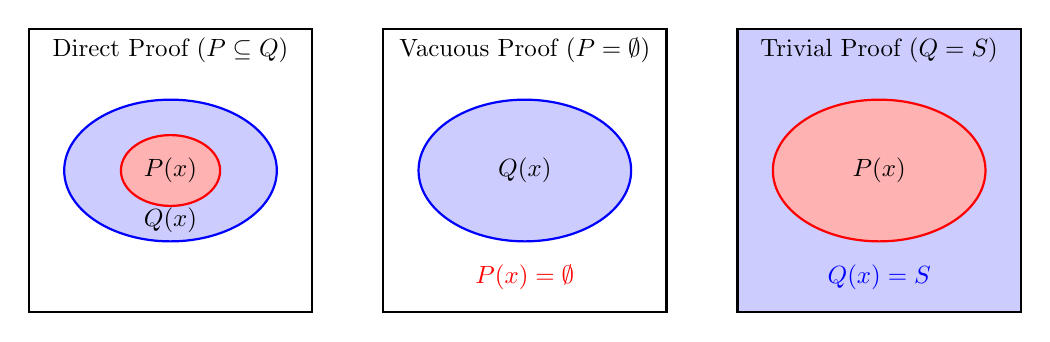
\begin{tikzpicture}[scale=0.9, every node/.style={transform shape}]
    % Direct Proof
    \begin{scope}[xshift=0cm]
        \draw[thick] (0,0) rectangle (4,4);
        \node at (2, 3.7) {Direct Proof ($P \subseteq Q$)};
        \filldraw[fill=blue!20, draw=blue, thick] (2,2) ellipse (1.5cm and 1cm);
        \filldraw[fill=red!30, draw=red, thick] (2,2) ellipse (0.7cm and 0.5cm);
        \node at (2,2) {$P(x)$};
        \node at (2, 1.3) {$Q(x)$};
    \end{scope}
    
    % Vacuous Proof
    \begin{scope}[xshift=5cm]
        \draw[thick] (0,0) rectangle (4,4);
        \node at (2, 3.7) {Vacuous Proof ($P = \emptyset$)};
        \filldraw[fill=blue!20, draw=blue, thick] (2,2) ellipse (1.5cm and 1cm);
        \node at (2,2) {$Q(x)$};
        \node[red, font=\bfseries] at (2, 0.5) {$P(x) = \emptyset$};
    \end{scope}

    % Trivial Proof
    \begin{scope}[xshift=10cm]
        \draw[thick, fill=blue!20] (0,0) rectangle (4,4);
        \node at (2, 3.7) {Trivial Proof ($Q = S$)};
        \filldraw[fill=red!30, draw=red, thick] (2,2) ellipse (1.5cm and 1cm);
        \node at (2,2) {$P(x)$};
        \node[blue, font=\bfseries] at (2, 0.5) {$Q(x) = S$};
    \end{scope}
\end{tikzpicture}
\end{center}

\subsection{Heuristics \& "Cheats"}
\begin{itemize}
    \item \textbf{Check the extreme cases first:} If an implication looks absurd or too complex, plug in the extreme bounds of the domain (e.g., $n=1$ for $\mathbb{N}$, or $n=0$ for $\mathbb{Z}$). If $P(x)$ is false at the extremes, suspect a Vacuous Proof.
    \item \textbf{Look for Squares:} If you see a polynomial of degree 2 that does not easily factor, immediately complete the square. It instantly reveals the global minimum/maximum of the function.
    \item \textbf{The $2m+1$ target:} When trying to prove an expression is odd, do not let large constants confuse you. Extract all even numbers and group them, leaving a lone $+1$ or $-1$ at the end.
\end{itemize}

\subsection{Pitfalls \& Fallacies}
\begin{itemize}
    \item \textbf{Domain Blending:} Assuming variables are Reals when defined as Integers. A classic mistake in parity proofs is writing $x = 2k+1$ but forgetting to state $k \in \mathbb{Z}$. Without $k \in \mathbb{Z}$, \textit{any} real number could be "odd" (e.g., $2.5 = 2(0.75) + 1$).
    \item \textbf{Affirming the Consequent:} Proving $Q(x)$ is true for a specific $x$, and assuming that means $P(x) \implies Q(x)$ is proven. 
    \item \textbf{False Vacuous Assertions:} Concluding an implication is vacuously true because you couldn't find a solution to $P(x)$. You must mathematically \textit{prove} $P(x)$ has no solutions over the domain.
\end{itemize}

\newpage
% =======================================================================
\section{Part 5: Conceptual Synthesis and The "Big Picture"}
% =======================================================================

\subsection{A) Thematic Connections}
The central unifying theme of these sections is the rigorous establishment of \textbf{conditional domains}. In pure mathematics, an implication $P \implies Q$ is essentially a localized theorem: "Within the universe $S$, if we restrict our attention solely to the subspace where $P$ holds, does $Q$ also hold?" 

This framework is deeply connected to \textit{measure theory}. In probability, a conditional probability $\mathbb{P}(A | B) = \frac{\mathbb{P}(A \cap B)}{\mathbb{P}(B)}$ is undefined in basic probability if $\mathbb{P}(B) = 0$. However, in measure-theoretic logic, events of measure zero act like vacuously false premises. By strictly defining behavior in null sets, mathematicians prevent logical paradoxes in stochastic integration (e.g., Itô integrals are defined "almost surely"). The vacuous proof is the discrete logic equivalent of an "almost sure" property where the failure set is exactly the empty set.

\subsection{B) Forward and Backward Links}
\begin{itemize}
    \item \textbf{Backward Link:} This material formalizes introductory set theory. The truth set of $P \implies Q$ is equivalent to asserting that $\{x \in S : P(x)\} \subseteq \{x \in S : Q(x)\}$. 
    \item \textbf{Forward Link:} Understanding parity (even/odd) and direct proofs forms the foundation for \textit{Modular Arithmetic} (congruences modulo $n$), which is the basis for cryptography (RSA encryption). Furthermore, vacuous truth is an essential mechanism in \textit{Mathematical Induction}. The base case often relies on a trivial or direct proof, while the inductive step ($P(k) \implies P(k+1)$) is an implication that must be proved logically sound regardless of whether $P(k)$ is actually true globally.
\end{itemize}

% =======================================================================
\section{Part 6: Abstract Real-World Modeling (AI, ML, \& Quant Finance)}
% =======================================================================

\subsection{A) Concrete Scenarios}
\begin{enumerate}
    \item \textbf{Algorithmic Verification in Autonomous AI:} In safety-critical AI (e.g., self-driving cars, nuclear reactor control), verification frameworks like Hoare logic use implications. An assertion $\{P\} \ C \ \{Q\}$ means "If precondition $P$ holds, execution of code $C$ results in postcondition $Q$." If an AI module's precondition $P$ is rigorously proven to be physically impossible (a vacuous proof), the system architect can trivially guarantee the postcondition constraint is never violated, saving massive computational overhead.
    \item \textbf{Arbitrage-Free Pricing in Quantitative Finance:} In mathematical finance, the Fundamental Theorem of Asset Pricing relies on the assumption of No-Arbitrage. If $P(\omega)$ is the statement "strategy $\omega$ yields risk-free profit with zero initial investment", an arbitrage-free market implies $P(\omega)$ is false for all $\omega$. Consequently, any theorem about arbitrage strategies is vacuously true, allowing quantitative analysts to uniquely price derivatives using equivalent martingale measures without paradoxes.
\end{enumerate}

\subsection{B) Model Problem Setup: Formal Verification of AI Constraint Sets}
\textbf{The Scenario:} Consider a generative AI model that outputs an embedding vector $x \in \mathbb{R}^d$. To prevent toxic or out-of-bound outputs, a safety filter applies a constraint: $P(x): \|x\|_2^2 - 2 \langle x, \mu \rangle + \|\mu\|_2^2 < 0$, where $\mu$ is an anchor vector. If an output triggers $P(x)$, a highly computationally expensive fallback protocol $Q(x)$ is initiated. 

\textbf{Mathematical Formulation:} 
Let $x, \mu \in \mathbb{R}^d$. The system requires computing:
\[ \forall x \in \mathbb{R}^d, \ P(x) \implies Q(x) \]
The engineering team wants to prove they never need to allocate GPU memory for the fallback protocol $Q(x)$.
\begin{proof}[Quantitative Model Proof]
Observe the left side of the inequality in $P(x)$:
\[ \|x\|_2^2 - 2 \langle x, \mu \rangle + \|\mu\|_2^2 \]
By the properties of the standard Euclidean inner product space, this is exactly the expansion of the squared $L_2$ norm of the difference vector:
\[ \|x - \mu\|_2^2 = \|x\|_2^2 - 2 \langle x, \mu \rangle + \|\mu\|_2^2 \]
Thus, the condition $P(x)$ is equivalent to $\|x - \mu\|_2^2 < 0$. 
By the positive-definite axiom of norm spaces, $\|v\|_2 \ge 0$ for all $v \in \mathbb{R}^d$, which implies $\|v\|_2^2 \ge 0$.
Therefore, $\|x - \mu\|_2^2 < 0$ is logically impossible. 
The set of trigger conditions $S = \{x \in \mathbb{R}^d : P(x) \text{ is true}\} = \emptyset$.
By the principle of vacuous truth, the implication $P(x) \implies Q(x)$ holds vacously, and the probability measure of triggering the fallback $\mathbb{P}(P(X)) = 0$. The firm safely deletes the code for $Q(x)$.
\end{proof}

\newpage
% =======================================================================
\section{Part 7: Common Variations and Untested Concepts}
% =======================================================================

While the provided homework covers parity and quadratic inequalities, advanced undergraduate courses often introduce \textbf{Divisibility} and \textbf{Rational numbers} in the introductory direct proofs section.

\subsection{Variation 1: Divisibility proofs}
\begin{definition}[Divisibility]
For integers $a$ and $b$ (with $a \neq 0$), we say $a$ divides $b$, denoted $a \mid b$, if there exists an integer $k$ such that $b = ak$.
\end{definition}

\textbf{Missing Concept Theorem:} Prove that if $a \mid b$ and $a \mid c$, then for any integers $x$ and $y$, $a \mid (bx + cy)$.
\begin{proof}[Direct Proof]
Assume $a, b, c \in \mathbb{Z}$ with $a \neq 0$, and assume $a \mid b$ and $a \mid c$. 
By definition, there exist integers $k, m \in \mathbb{Z}$ such that $b = ak$ and $c = am$. 
Let $x, y \in \mathbb{Z}$ be arbitrary integers. We examine the linear combination $bx + cy$:
\[ bx + cy = (ak)x + (am)y \]
Using the associative and distributive properties of integers:
\[ bx + cy = a(kx) + a(my) = a(kx + my) \]
Let $j = kx + my$. Because integers are closed under multiplication and addition, $j \in \mathbb{Z}$. 
Thus, $bx + cy = aj$. By definition of divisibility, $a \mid (bx + cy)$.
\end{proof}

\subsection{Variation 2: Direct proofs with Rational Numbers}
\begin{definition}[Rational Number]
A real number $r$ is rational, denoted $r \in \mathbb{Q}$, if there exist integers $p, q \in \mathbb{Z}$ with $q \neq 0$ such that $r = \frac{p}{q}$.
\end{definition}
\textbf{Missing Concept Theorem:} Prove that the sum of two rational numbers is rational.
\begin{proof}[Direct Proof]
Assume $x, y \in \mathbb{Q}$. By definition, there exist integers $a, b, c, d$ with $b \neq 0$ and $d \neq 0$ such that $x = \frac{a}{b}$ and $y = \frac{c}{d}$.
Consider their sum:
\[ x + y = \frac{a}{b} + \frac{c}{d} = \frac{ad + bc}{bd} \]
Let $p = ad + bc$ and $q = bd$. Since integers are closed under addition and multiplication, $p, q \in \mathbb{Z}$. 
Since $b \neq 0$ and $d \neq 0$, the Zero Product Property implies $q = bd \neq 0$.
Thus, $x + y = \frac{p}{q}$ where $p,q \in \mathbb{Z}$ and $q \neq 0$. By definition, $x + y \in \mathbb{Q}$.
\end{proof}

\newpage
% =======================================================================
\section{Part 8: Advanced Diagnostic Testing: "Find the Flaw"}
% =======================================================================

Below are 5 proposed theorems and their proofs. Each proof looks rigorous at first glance but contains a fatal, subtle logical or mathematical error related to definitions, variables, or proof structure.

\textbf{Problem 1:} 
\textit{Theorem:} Let $x, y \in \mathbb{Z}$. If $x$ and $y$ are both even, then $x + y$ is a multiple of $4$.
\begin{proof}[Proposed Proof]
Assume $x$ and $y$ are even integers. By definition of an even integer, we can write $x = 2k$ and $y = 2k$ for some integer $k \in \mathbb{Z}$. Adding the two equations together yields $x + y = 2k + 2k = 4k$. Since $k$ is an integer, $x+y$ is a multiple of $4$.
\end{proof}

\textbf{Problem 2:} 
\textit{Theorem:} Let $x \in \mathbb{C}$ (complex numbers). If $x^2 < 0$, then $x^3 = 5$.
\begin{proof}[Proposed Proof]
We use a vacuous proof. The hypothesis states that $x^2 < 0$. However, we know that the square of any number is always non-negative (i.e., $x^2 \ge 0$). Therefore, the hypothesis is logically impossible. Since the hypothesis is false for all $x$, the implication is vacuously true.
\end{proof}

\textbf{Problem 3:}
\textit{Theorem:} Let $x \in \mathbb{R}$. If $x > 10$, then $x^2 \ge 0$.
\begin{proof}[Proposed Proof]
We will prove this via a trivial proof. The hypothesis is $P(x) : x > 10$. The conclusion is $Q(x) : x^2 \ge 0$. Since $x > 10$, we can multiply both sides by $x$ (which is positive) to get $x^2 > 10x$. Since $x > 10$, $10x > 100$. Thus $x^2 > 100 \ge 0$. Thus $Q(x)$ is true. Because $Q(x)$ is true, the proof is trivially complete.
\end{proof}

\textbf{Problem 4:}
\textit{Theorem:} Let $x \in \mathbb{Z}$. If $x^2$ is even, then $x$ is even.
\begin{proof}[Proposed Proof]
Assume $x$ is an even integer. By definition, $x = 2k$ for some integer $k \in \mathbb{Z}$. We evaluate $x^2$: $x^2 = (2k)^2 = 4k^2 = 2(2k^2)$. Let $m = 2k^2$. Since $k \in \mathbb{Z}$, $m \in \mathbb{Z}$. Thus $x^2 = 2m$, which means $x^2$ is even. This concludes the direct proof.
\end{proof}

\textbf{Problem 5:}
\textit{Theorem:} Let $x \in \mathbb{Z}$. If $2x = x^2 + 1$, then $x$ is odd.
\begin{proof}[Proposed Proof]
Assume $2x = x^2 + 1$. Rearranging this equation gives $x^2 - 2x + 1 = 0$, which factors as $(x-1)^2 = 0$. The only solution to this in $\mathbb{Z}$ is $x = 1$. Since $x=1$ can be written as $2(0) + 1$, and $0 \in \mathbb{Z}$, $x$ is an odd integer. The proof is complete. (But what is the structural flaw?)
\end{proof}

\vspace{0.5cm}
\hrule
\vspace{0.5cm}

\subsection{Solution Key: Flaw Resolutions}

\textbf{Resolution 1:} 
\textit{Flaw:} Variable aliasing. The proof uses the same dummy variable $k$ for both $x$ and $y$. This implicitly assumes $x = y$, which is not stated in the theorem. 
\textit{Correction:} Use distinct variables. Let $x = 2k$ and $y = 2m$ for $k,m \in \mathbb{Z}$. Then $x+y = 2k+2m = 2(k+m)$. This only proves $x+y$ is even, not a multiple of 4. (Indeed, $2+6=8$ is a multiple of 4, but $2+4=6$ is not).

\textbf{Resolution 2:}
\textit{Flaw:} Misapplying real number axioms to the complex domain. The axiom $x^2 \ge 0$ only holds for $x \in \mathbb{R}$. In $\mathbb{C}$, if $x = i$, then $x^2 = -1 < 0$. Thus the hypothesis is NOT always false. 
\textit{Correction:} The theorem is actually false. For $x = i$, $x^2 < 0$ is true, but $i^3 = -i \neq 5$, so the implication is false.

\textbf{Resolution 3:}
\textit{Flaw:} Misunderstanding the definition of a Trivial Proof. A trivial proof requires showing $Q(x)$ is \textit{always} true over the \textit{entire domain} $\mathbb{R}$, independent of $P(x)$. The proof provided used the hypothesis $x > 10$ to derive $Q(x)$. 
\textit{Correction:} This was a Direct Proof disguised in bad terminology. To actually use a trivial proof, state: "By the axioms of real numbers, $x^2 \ge 0$ for ALL $x \in \mathbb{R}$. Because $Q(x)$ is universally true, the implication is trivially true, ignoring $x>10$ entirely."

\textbf{Resolution 4:}
\textit{Flaw:} Affirming the consequent / Proving the converse. The theorem requires proving $x^2 \text{ is even} \implies x \text{ is even}$. The proof started by assuming $x$ is even, and concluded $x^2$ is even. 
\textit{Correction:} A direct proof for this is difficult. One should use a Proof by Contrapositive (assume $x$ is odd, show $x^2$ is odd), which is covered in the next section (3.3).

\textbf{Resolution 5:}
\textit{Flaw:} There is no mathematical error, but the structure strictly limits the domain to $x=1$. Because $(x-1)^2 = 0 \implies x=1$, it turns out $P(x)$ is ONLY true when $x=1$. While the proof correctly evaluates the singular case, it feels like solving an equation rather than proving a property.
\textit{Correction:} While technically a valid direct proof, it is highly degenerate. It borders on proving something specific to a single constant rather than an arbitrary variable. A more general approach is often required, though valid here due to the extreme constraint of the hypothesis.

\end{document}